\begin{figure}
%\centering
\begin{subfigure}[b]{0.25\textwidth}
\centering
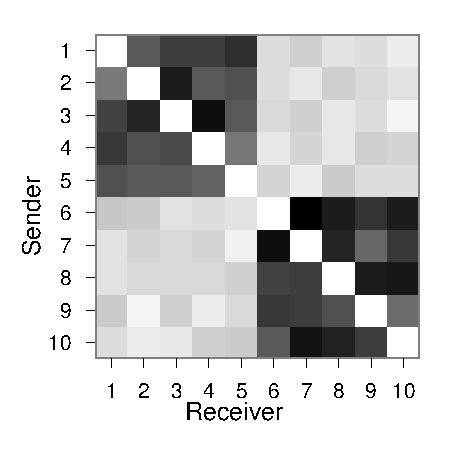
\includegraphics[width=1.5in]{../figs/synthetic/mat.pdf} %counts2.pdf
\vspace{.25cm}
\caption{}
\end{subfigure}
~
\begin{subfigure}[b]{0.3\textwidth}
\centering
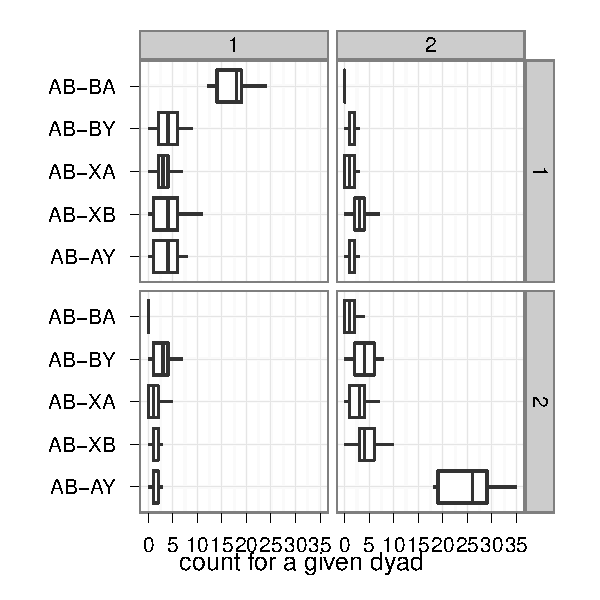
\includegraphics[width=2in]{../figs/synthetic/counts.pdf}
\caption{}
\end{subfigure}
~
\begin{subfigure}[b]{0.3\textwidth}
\centering
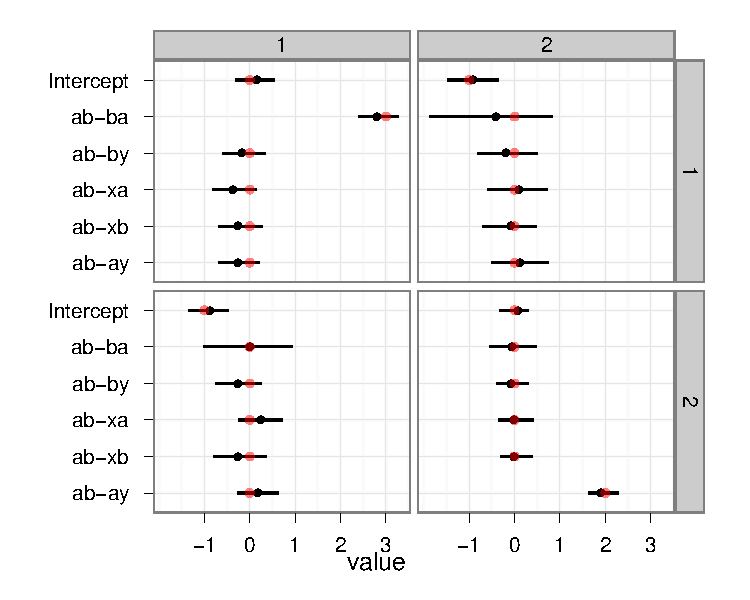
\includegraphics[width=2.1in]{../figs/synthetic/params-estimates.pdf}
\vspace{-.5cm}
\caption{}
\end{subfigure}
\caption{Illustration of 2000 simulated events, as described in text. (a) Counts of each dyad. (b) Boxplot of distribution of participation counts across dyads.  The top left shows an increased propensity for reciprocity within cluster 1; bottom right shows more AB-AY events within cluster 2.  (c) Parameters (in red) and posterior credible intervals (in black).}
\label{fig:syncounts}
\end{figure}

\section{Simulation}
\label{sec:simulation}

We check our model fitting procedure using a small synthetic data set involving 10 nodes from 2 groups where 1) within group communication is more likely, 2) events among members in the first group are more likely to be reciprocated  (i.e. a positive \texttt{ab-ba} effect), and 3) events among members of the second group are more likely to be followed by an event with the same sender (i.e. a positive \texttt{ab-ay} effect).  The specification of $\textbf{s}$ is therefore $\textbf{s}(t,i,j,\mathcal{A}_t) = [s_0, s_{1}(t,i,j,\mathcal{A}_t), s_{2}(t,i,j,\mathcal{A}_t)]$.  For the synthetic data set we use parameter vectors $\boldsymbol{\beta}_{1,1} = (0,3,0)$,  $\boldsymbol{\beta}_{1,2} = \boldsymbol{\beta}_{2,1} = (-1,0,0)$, and $\boldsymbol{\beta}_{2,2} = (0,2,0)$.
Data is generated by sequentially computing $\lambda_{ij}(t_m|\cdot)$ for all $(i,j) \in \mathcal{R}$, drawing $t_{m+1}-t_m \sim \mbox{Exp}(\sum_{ij} \lambda_{ij}(t_m|\cdot))$, and drawing the dyad $(i,j) \sim \mbox{Categorical}(\lambda_{ij}(t_m|\cdot) / \sum_{ij}\lambda_{ij}(t_m|\cdot))$.

Though the dyad counts for the synthetic data set suggest a stochastic blockmodel (as seen in Figure  \ref{fig:syncounts}),  the center plot shows each block has empirical differences in their dynamics.
Intensities for reciprocal actions among nodes in block 1 are $e^3 \approx 20$ times greater, intensities for turn-taking actions among nodes in group 2 are $e^2$ times greater, and intensities for dyadic interactions between the two groups have a multiplicative effect of $e^{-1}$ and thus occur less often.
Fitting the model with $K=2$ has similar  predictive accuracy as the true model (see Table \ref{tab:results}), recovers the true latent classes, and the posterior credible intervals of the parameters cover the true parameter values (see Figure \ref{fig:syncounts}c).
